A comparison between the dynamic state estimation of a Luenberger observer and the algebraic recovery of both state and disturbance of the projection filtering method is given in Example 1. Noise is added in Example 2, in order to showcase that the projection filtering method is able to handle noise in measurements, by the cost of an additional sensor. 
\subsection{Example 1}
The electrical system given in\cite{yang2025output} with parameters $C_t=2.2\mathrm{mF}$, $L_t=1.8\mathrm{mH}$ and $R_t=0.2\Omega$ is defined as the following state space model,
\begin{equation}
A=\begin{bmatrix}
    0& \frac{1}{C_t}\\
    -\frac{1}{L_t}& -\frac{-R_t}{L_t}    
\end{bmatrix},\,
B_w=\begin{bmatrix}
    -\frac{1}{C_t}\\
    0    
\end{bmatrix},\,
C=\begin{bmatrix}
    1& 0\\    
    1& 0\\    
    0& 1    
\end{bmatrix}
\end{equation}
where output redundancy is created by replicating the sensor measuring first state. The exogenous input matrix is constructed as follows,
\begin{equation}
    D_w=C^\perp+C\begin{bmatrix}1\\1\end{bmatrix}=\begin{bmatrix}
    1.7071\\
    0.2929\\
    1.0000
    \end{bmatrix}
\end{equation}
A Luenberger observer is designed solving the LMI given in (\ref{eqn:lmi1}) assuming $C_z=I$. Solving the corresponding LMI, yields,
\begin{equation}
    Y=\begin{bmatrix}
 -159314.9& 7541099.0& -12347840.0\\
-1741760.0& 3556493.0&   3485615.0
    \end{bmatrix}
\end{equation}
and
\begin{equation}
    Z=\begin{bmatrix}
    0.0000449847& 0.00000887586\\
    0.00000887586&  0.0000594674
    \end{bmatrix}
\end{equation}
with $\gamma_\infty=0.0012$, $\gamma_2=0.0001044$. The observer gain and Lyapunov matrix are determined as,
\begin{equation}
    L=\begin{bmatrix}
    -22.6263&  370.8001& -524.5247\\
    -104.9918&  278.4287&   97.6824
    \end{bmatrix}
\end{equation}
and 
\begin{equation}
    P=\begin{bmatrix}
    22904.36& -3418.62\\
    -3418.62&  17326.22
    \end{bmatrix}
\end{equation}
noting that $B_w-LD_w=0$ is satisfied, hence the state estimation is not affected by the exogenous input. No assumption about the exogenous input is added, thus the estimated state is utilized to obtain the exogenous input with,
\begin{equation}
    \hat{w}=D_w^\dagger(y-Cx)
\end{equation}

On the other hand, using PFM the projection matrix given by Theorem~1 is determined for $C$ as,
\begin{equation}
\Pi^C=\begin{bmatrix}
    0.5&   -0.5&         0\\
    -0.5&    0.5&         0\\
    0&        0&         0
\end{bmatrix}
\end{equation}
and for $D_w$ as,
\begin{equation}
\Pi^{D_w}=\begin{bmatrix}
    0.2714&   -0.1250&   -0.4268\\
   -0.1250&    0.9786&   -0.0732\\
   -0.4268&   -0.0732&    0.7500\\
\end{bmatrix}
\end{equation}
The disturbance and the states are filtered using (\ref{eqn:filtering_w}) and (\ref{eqn:filtering_x}), respectively.
The state estimation and the projection state filtering is compared in Figure~\ref{fig:ex1_states1}.
\begin{figure}[!htb]
    \centering
    
\includegraphics[width=0.85\linewidth]{img/ex1_states1}
    \caption{Comparison of the Luenberger observer state estimation versus projection filtering state reconstruction.}
    \label{fig:ex1_states1}
\end{figure}

The estimation process of the Luenberger observer takes $0.01$ seconds due to the fact that the observer is a dynamic observer, whereas the projection filtering directly matches the original system states at $t=0$ seconds as illustrated in Figure~\ref{fig:ex1_states1}. It is possible to decrease the estimation duration of the observer by speeding up the observer eigenvalues, but in return the observer gain and therefore noise amplification would increase. 


% The exogenous input estimated and filtered is depicted in Figure~\ref{fig:ex1_disturbance}.
\begin{figure}[!htb]
    \centering
    
\includegraphics[width=0.85\linewidth]{img/ex1_disturbance}
    \caption{Estimated disturbance using Luenberger Observer versus reconstructed disturbance of the projection filtering}
    \label{fig:ex1_disturbance}
\end{figure}

The Luenberger observer is a state estimator, but using the linear mapping of the output, it is possible to reconstruct the disturbance assuming the lack of noise in the measured output. It also possible to employ a Disturbance Observer, but then it is necessary to also assume a certain model or add an assumption about the disturbance. This extra information about the disturbance is not necessary for the projection filtering method. 
As illustrated in Figure~\ref{fig:ex1_disturbance}, the reconstruction of the disturbance using the Luenberger observer state matches the disturbance only in the steady state, since the state estimation gets corrected during the transients. But, the projection filtering method results in an exact match, due to its static approach.


% The projection filtering method utilizes the geometric properties of the output mapping, hence no dynamic estimation is present, it directly extracts the output map into its components. Despite the fact that the Luenberger observer gain for output redundant systems is able to eliminate the exogenous input term in the error dynamic by setting $B_w-LD_w$ to zero, the structure exploit performs better for the given example since no estimation takes place. Static output filtering fails if 
% \begin{equation}
%     D_w=C\alpha
% \end{equation}
% since,
% \begin{equation}
%     \Pi y=\Pi Cx+\Pi D_w w=\Pi C(x+\alpha)=0
% \end{equation}
% which shows that different channels need to exist in order separate signals using the projection. 

\subsection{Example 2}
In most practical applications noise is present in measured outputs as given in,
\begin{equation}
    y=Cx+D_w w+D_n n\label{eqn:ex2_output_mapping1}
\end{equation}
For illustrative purposes the following output equation is defined
\begin{equation}
    y=\begin{bmatrix}
    1&     0\\
    2&     1\\
    0&     1\\
    0&     1
    \end{bmatrix}x(t)+\begin{bmatrix}
        2.2060\\
        2.3970\\
        1.3015\\
        1.3015
    \end{bmatrix}w(t)+
    \begin{bmatrix}
    0.1960\\
    0.7382\\
    0.6697\\
    0.5265
    \end{bmatrix}n(t)
\end{equation}
where $w(t)$ is disturbance, $n(t)$ is noise and $x(t)$, which represent some system states and  are arbitrarily chosen as,
\begin{equation}
    x(t)=\begin{bmatrix}
        \sin(t)\\ \cos(t)
    \end{bmatrix}
\end{equation}
In order to be able to recover both the states and the disturbance in such a system, the number of sensors for measurement needs to increase, otherwise, the least square estimation will be the only recovery attainable. 

The disturbance matrix is defined using 
\begin{equation}
    D_w=C\begin{bmatrix}1\\1\end{bmatrix}+C^\perp\begin{bmatrix}1\\1\end{bmatrix}
\end{equation}
and the noise matrix $D_n$ is chosen as a random matrix.

The output mapping in (\ref{eqn:ex2_output_mapping1}) is rewritten as,
\begin{equation}
    y=Cx+\begin{bmatrix}
        D_w& D_n
    \end{bmatrix}\begin{bmatrix}
    w\\n        
    \end{bmatrix}
\end{equation}
and the projection defined using Corollary~1.2 to recover the state information $x(t)$ can be calculated using,
\begin{equation}
    \Pi^{wn}=I-\begin{bmatrix}
        D_w& D_n
    \end{bmatrix}\left(
        \begin{bmatrix}
        D_w\\ D_n
    \end{bmatrix}\begin{bmatrix}
        D_w& D_n
    \end{bmatrix}
    \right)^{-1}\begin{bmatrix}
        D_w\\D_n
    \end{bmatrix}
\end{equation}
and is determined as
\begin{equation}
    \Pi^{wn}=\begin{bmatrix}
    0.6224&   -0.2581&   -0.3034&   -0.2763\\
    -0.2581&    0.1118&    0.1698&    0.0618\\
    -0.3034&    0.1698&    0.5564&   -0.3549\\
    -0.2763&    0.0618&   -0.3549&    0.7094
    \end{bmatrix}
\end{equation}
Then the state $x(t)$ is recovered using,
\begin{equation}
    \hat{x}=(\Pi^{wn}C)^\dagger (\Pi^{wn}y)
\end{equation}

\begin{figure}[!htb]
    \centering
    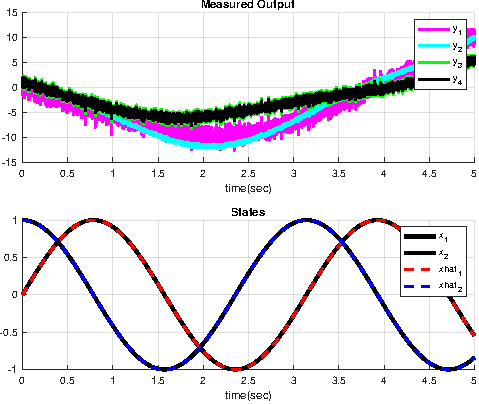
\includegraphics[width=0.85\linewidth]{img/ex2_results}
    \caption{The measured outputs($y_1$, $y_2$, $y_3$, $y_4$) and the states($x_1$, $x_2$) versus the projection filtering method recovered states($\hat{x}_1$, $\hat{x}_2$)}
    \label{fig:ex2_results}
\end{figure}
The measured output for each sensor with noise is depicted in Figure~\ref{fig:ex2_results}. The output redundancy can be observed by comparing third output and fourth output in Figure~\ref{fig:ex2_results}. It can also be seen that the projection filtering method is able to reconstruct both states under noisy measurements.


The disturbance is recovered using the projection on $\begin{bmatrix}
        C& D_n
    \end{bmatrix}$ as,
\begin{gather}
    \Pi^{xn}=\begin{bmatrix}
     0.7254&   -0.3627&    0.1507&    0.2120\\
   -0.3627 &   0.1813 &  -0.0754 &  -0.1060\\
    0.1507 &  -0.0754 &   0.0313 &   0.0440\\
    0.2120 &  -0.1060 &   0.0440 &   0.0619
    \end{bmatrix}
\end{gather}
and is plotted in Figure~\ref{fig:ex2_results2}. It is observed that disturbance recovery works in a similar fashion compared to state recovery in Figure~\ref{fig:ex2_results}. 

\begin{figure}[!htb]
    \centering
    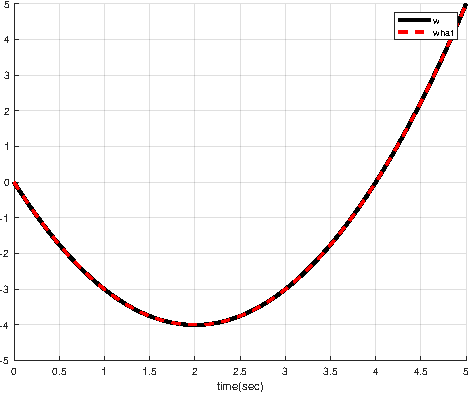
\includegraphics[width=0.85\linewidth]{img/ex2_results2}
    \caption{Disturbance recovered by projection filtering versus actual disturbance}
    \label{fig:ex2_results2}
\end{figure}


Throughout the examples given in this section, it has been established that, the projection filtering method exploits the output mapping using a projection matrix and recovers the states and the disturbance of a system directly. Whereas, the Luenberger observer, however fast dynamics it possesses, estimates the states of a system, due to its dynamic structure. Assuming no information about disturbance, one can also back-calculate the disturbance in a system with the Luenberger state estimates. Due to the dynamics, the disturbance and state estimations are valid for steady-state. But projection filtering gives valid results for both transient and steady-state regime. Additionally, projection filtering can handle noise, if necessary amount of sensors are present. 